\documentclass[journal]{IEEEtran}

\usepackage[T1]{fontenc}
\usepackage{amsmath,amssymb}
\usepackage{booktabs}
\usepackage{cite}
\usepackage{graphicx}
\usepackage{multirow}
\usepackage{siunitx}
\usepackage{xcolor}
\usepackage[hidelinks]{hyperref}
\usepackage{balance}

\graphicspath{{figures/}%
{../../../artifacts/tx3/E03_E04/figures/}%
{../../../artifacts/tx3/E05_mechanism_consequence/figures/}%
{../../../artifacts/tx3/E05B_dynamic_spectral_shift/figures/}%
{../../../artifacts/tx3/E05C_margin_conditioned/figures/}%
{../../../artifacts/tx3/critical_mode_baseline_audit/figures/}}

\newcommand{\ext}[1]{\Delta_{#1}}
\newcommand{\RR}{\mathbb{R}}
\newcommand{\CC}{\mathbb{C}}
\newcommand{\tr}{\operatorname{tr}}
\newcommand{\Part}{\operatorname{Part}}

\title{Finite Connected Externalities in Converter-Rich Power-System
Dynamics: Re-Equilibrated Reconstruction, Pole Anatomy, and the Boundary of
Modal Materiality}

\author{Authors withheld for double-blind review}

\begin{document}
\maketitle

\begin{abstract}
Engineering actions in converter-rich grids are commonly screened one at a
time or through local sensitivities. Such calculations do not isolate the
finite non-additive effect of a portfolio after its operating point has moved.
This paper formulates a connected intervention calculus for finite actions on
an index-one differential--algebraic power-system model. Every coalition is
solved at its own ac equilibrium, reinitialized, and rebuilt before a
band-integrated relative log-determinant is evaluated. Pair and triple
M\"obius externalities are reconstructed independently from connected total
derivatives over the action hypercube. In a matched IEEE 39-bus benchmark with
three grid-following converters, 266 of 672 pair cases and 147 of 1,344 triple
cases exceeded five conservative uncertainty budgets. All 129 locked-holdout
reconstructions closed within the same five-budget criterion. An exact Schur
factorization then separates algebraic, mass-scaling, and finite-pole terms;
its largest closure error is $7.39\times10^{-13}$. For the leading dispatch--
network pair, a frozen-affine calculation underestimates the finite effect by
approximately $6.3\times$ at the OP00 reference point. Yet the strongest
externalities are concentrated in well-damped converter-control modes, whereas
the actual limiting mode is a $1.22$-Hz synchronous-electromechanical mode.
Across all 15 retained coalitions, the largest baseline critical-mode damping
externality is only $5.15\times10^{-6}$. Thus a reproducible dynamic
externality can exist without materially consuming the registered damping
margin. This distinction defines both the contribution and the limit of the
method: it diagnoses finite interaction structure, but is not by itself a
stability or mitigation certificate.
\end{abstract}

\begin{IEEEkeywords}
converter-driven stability, differential--algebraic equations, eigenvalue
analysis, grid-following converters, higher-order interactions, M\"obius
inversion, power-system dynamics, spectral determinant
\end{IEEEkeywords}

\section{Introduction}
\IEEEPARstart{C}{onverter-rich} power systems couple controller parameters,
active-power schedules, and network conditions through both the ac operating
point and the dynamic Jacobian. The effect of changing two devices together
therefore need not equal the sum of changing them separately. This elementary
observation is operationally important: screening tools are frequently local
or one-action-at-a-time, while actual planning and tuning decisions arrive as
finite portfolios.

Several mature theories already illuminate parts of this problem. Classical
modal analysis relates states, residues, participations, and eigenvalue
sensitivities to oscillatory behavior
\cite{perezarriaga1982sma,pagola1989sensitivities}. Augmented and
multi-parameter sensitivities can retain equilibrium dependence and
higher-order terms \cite{nam2000eigensensitivity,zamoracardenas2013multiparameter}.
Return-ratio and impedance methods expose feedback interactions without
requiring the same internal coordinate description
\cite{macfarlane1970return,sun2011impedance,rygg2016sequence}. Recent work
also uses open-loop modal proximity and second-order eigenvalue displacement to
identify converter interaction modes \cite{dewangan2026interaction}.

These methods answer valuable but different questions. A derivative is local
to its expansion point. An impedance or return-ratio criterion evaluates a
feedback interconnection. A participation factor associates a mode with
states. None of these objects, by itself, is the finite inclusion--exclusion
remainder of a specified engineering portfolio after every subset has been
physically applied and independently re-equilibrated. The combinatorial
operation needed to isolate that remainder is M\"obius inversion
\cite{rota1964mobius,grabisch1997kadditive}. The missing bridge is to apply it
to a re-equilibrated differential--algebraic operator and then connect the
finite result to derivative, factor, and modal descriptions without confusing
existence with consequence.

This paper develops and tests that bridge. A normalized action coordinate
maps zero to a registered baseline and one to a finite engineering change.
For each coalition vertex, the ac power flow is solved again, dynamic states
are initialized again, and the descriptor operator is rebuilt. A relative
real log-determinant, integrated over a fixed frequency band, summarizes the
resulting operator. Direct pair and triple M\"obius differences define the
finite externality. Independently, a connected set-partition formula
integrates mixed total derivatives over the action hypercube. The two routes
must close within a case-specific uncertainty budget.

The contribution is not a new M\"obius identity, Schur complement, trace
formula, perturbation determinant, or eigenvalue sensitivity. It is the
following integrated, experimentally gated workflow:
\begin{enumerate}
    \item a finite set function whose every vertex is an independently
    re-equilibrated power-system DAE;
    \item a connected reconstruction that retains mixed physical and
    equilibrium curvature rather than only singleton feedback;
    \item an exact descriptor-factor anatomy separating algebraic,
    mass-scaling, and finite-pole externalities;
    \item a registered modal-materiality ladder that asks whether the
    externality reaches the mode that actually sets the damping margin.
\end{enumerate}

Table~\ref{tab:methods} makes the novelty perimeter explicit. The first four
rows are established approaches; none is displaced here. M\"obius inversion
supplies the set-function coefficient, higher-order sensitivity supplies local
derivative information, and return-ratio/impedance methods supply loop-level
stability information. The proposed contribution is the registered
combination of a finite re-equilibrated power-system set function, complete
pair/triple subset evaluation, connected reconstruction, descriptor-factor
anatomy, and a separate materiality test.

\begin{table*}[t]
\caption{Method-to-Method Novelty Perimeter}
\label{tab:methods}
\centering
\scriptsize
\begin{tabular}{p{0.17\textwidth}p{0.12\textwidth}p{0.16\textwidth}p{0.21\textwidth}p{0.19\textwidth}}
\toprule
Approach & Amplitude & Equilibrium treatment & Interaction object & Primary interpretation\\
\midrule
First-order eigen-sensitivity
& Local
& One expansion point
& Singleton derivative of a selected eigenvalue
& Directional modal change\\
Higher-order total sensitivity
& Local Taylor series
& May include implicit equilibrium derivatives
& Selected mixed derivatives to a truncation order
& Local curvature and parameter ranking\\
Return-ratio / impedance
& Frequency-domain model
& Operating point supplied to the model
& Ports, loops, or interconnection blocks
& Nyquist/loop stability and coupling\\
Proximal eigenvalue displacement \cite{dewangan2026interaction}
& First-/second-order modal displacement
& Not an all-subset finite-action requirement
& Proximal open-loop modal coupling
& Identification of converter interaction modes\\
M\"obius set-function coefficient
& Finite
& Domain-agnostic vertex values
& All subsets of a specified set
& Pure higher-order set-function dividend\\
This work
& Finite registered actions
& New AC solution and DAE at every required vertex
& All vertices of every registered pair and triple
& Externality, exact factor anatomy, then separate registered modal materiality\\
\bottomrule
\end{tabular}
\end{table*}

The tests use a canonical IEEE 39-bus system with three grid-following (GFL)
converters and eight moderate actions. The main positive result is numerical
and structural: reproducible pair and genuine third-order finite-pole
externalities exist, and the connected reconstruction closes the direct
finite computation. The main negative result is equally important: the
largest externalities found in the registered search do not materially alter
the limiting damping mode. A post-mortem identifies a family mismatch. The
externality-dominant modes are well-damped converter-control or
phase-locked-loop (PLL) modes, while the limiting mode is a lightly damped
synchronous-electromechanical mode. Hence \emph{dynamic externality existence
and operational interpretation under a registered modal-materiality screen
are distinct claims}.

This distinction narrows the practical interpretation. The calculus can tell
an analyst that a finite portfolio contains reproducible, non-additive dynamic
structure, quantify what a frozen model misses, and locate pole motion when a
contour certificate is valid. It does not certify instability, identify an
industrial mitigation, establish cycle or strongly connected component
(SCC) causality, or transfer a mechanism to electromagnetic-transient (EMT)
simulation. The cross-domain EMT work in this study validates only the matched
benchmark infrastructure used to launch the phasor-domain campaign.

The remainder of the paper is organized as follows. Section II defines the
finite calculus and exact factorization. Section III describes the registered
benchmark, actions, uncertainty budgets, and holdout discipline. Section IV
reports finite externalities and connected reconstruction. Section V separates
algebraic and pole contributions and presents contour localization. Section VI
reports the modal consequence and materiality boundary. Sections VII and VIII
discuss interpretation, limitations, and conclusions.

\section{Finite Connected Intervention Calculus}
\subsection{Actions and Re-Equilibrated Descriptor Operator}

Let $a=(a_1,\ldots,a_m)\in[0,1]^m$ denote normalized engineering actions.
Coordinate $a_i=0$ is the registered baseline and $a_i=1$ is the complete
finite action. Intermediate values provide a smooth interpolation; they are
not a first-order approximation. At every $a$, the ac equations are solved and
the dynamic model is reinitialized. Linearization of the resulting
differential--algebraic equations gives
\begin{equation}
T(s,a)=
\begin{bmatrix}
sM(a)-f_x(a) & -f_y(a)\\
-g_x(a) & -g_y(a)
\end{bmatrix},
\label{eq:descriptor}
\end{equation}
where $x$ and $y$ are differential and algebraic variables, respectively.
All derivatives in this paper are \emph{total} derivatives along the
re-equilibrated action path. They therefore contain direct parameter changes,
the implicit movement of the equilibrium, and the resulting Jacobian
curvature.

For a registered band $\Omega=[\omega_\ell,\omega_h]$ and fixed real
contour shift $\sigma$, define
\begin{equation}
\begin{aligned}
\Phi_\Omega(a)=\int_\Omega w(\omega)\big[&
\log|\det T(\sigma+j\omega,a)|\\
&-\log|\det T(\sigma+j\omega,0)|\big]\,d\omega .
\end{aligned}
\label{eq:phi}
\end{equation}
We use $w(\omega)=1/[\omega\log(\omega_h/\omega_\ell)]$, so
\eqref{eq:phi} is an average on logarithmic frequency. The baseline
subtraction makes $\Phi_\Omega(0)=0$. The real log-absolute determinant has
no complex-log branch choice. Fixed nonsingular left and right matrix
scalings add only action-independent constants and hence cancel in every
higher-order finite difference.

Equivalently, define the finite-dimensional relative determinant
$D(s,a)=\det T(s,a)/\det T(s,0)$ wherever the fixed contour is regular; then
the integrand in \eqref{eq:phi} is $\log|D(s,a)|$. This notation is only a
finite non-normal determinant ratio. Contour statements below follow from the
argument principle and registered numerical certificates, not from
self-adjoint spectral-shift theory.

The log determinant is used as a compact characteristic functional, not as a
standalone stability index. It aggregates how the full descriptor operator
changes across the selected frequency band. Its factor and modal
interpretations are tested later rather than assumed.

\subsection{Direct Finite Externality}

For a nonempty action set $S\subseteq\{1,\ldots,m\}$, let $1_U$ activate
exactly the subset $U\subseteq S$. The finite M\"obius externality is
\begin{equation}
\ext{S}\Phi=\sum_{U\subseteq S}(-1)^{|S|-|U|}\Phi(1_U).
\label{eq:mobius}
\end{equation}
For a pair, this is the joint response minus both singleton responses plus the
baseline. For a triple, it removes the three singleton and three pair
contributions. A nonzero triple coefficient is thus a genuine third-order
set-function dividend (M\"obius coefficient) in the chosen finite set
function. It is not, without additional
evidence, an irreducible three-device causal mechanism.

Equation \eqref{eq:mobius} is coordinate dependent in the ordinary sense that
the physical definition and amplitude of each action matter. It supports an
existential statement for the frozen actions, not a universal statement that
all portfolios or parameterizations are non-additive.

\subsection{Finite-to-Connected Bridge}

If the re-equilibrated map is sufficiently smooth on the full $|S|$-
dimensional hypercube, repeated application of the fundamental theorem of
calculus yields
\begin{equation}
\ext{S}\Phi
=\int_{[0,1]^{|S|}}\partial_S\Phi(a_S;a_{\bar S}=0)\, da_S .
\label{eq:bridge}
\end{equation}
This identity turns a vertex-level M\"obius coefficient into an integral of
a connected mixed derivative. It requires a smooth valid path, not merely
valid endpoints.

Write $G=T^{-1}$ and let $T_B$ be the mixed total derivative with labels in the
nonempty block $B\subseteq S$. Jacobi's identity and repeated product
differentiation give the complex connected derivative
\begin{equation}
\begin{aligned}
\partial_S\log\det T
={}&\sum_{\pi\in\Part(S)}\frac{(-1)^{k-1}}{k}\\[-2pt]
&\times\sum_{\rho\in\operatorname{Perm}(\pi)}
\tr\!\left(\prod_{r=1}^{k}GT_{B_{\rho(r)}}\right),
\end{aligned}
\label{eq:connected}
\end{equation}
where $\pi=\{B_1,\ldots,B_k\}$ is a set partition of $S$. The $1/k$
factor removes cyclic overcounting under the trace. The real part of
\eqref{eq:connected}, integrated over frequency and the action hypercube,
reconstructs \eqref{eq:mobius}. For a pair,
\begin{equation}
\partial_{12}\log\det T
=\tr(GT_{12})-\tr(GT_1GT_2),
\label{eq:pair}
\end{equation}
which explicitly separates mixed curvature from the familiar feedback
product. Triples contain intrinsic $T_{123}$, mixed-curvature/feedback, and
three-factor connected feedback terms. Omitting $T_{12}$ or higher mixed
terms is a frozen-affine diagnostic, not the finite calculus.

\subsection{Exact Descriptor-Factor Anatomy}

Assume the algebraic Jacobian $g_y(a)$ and the registered differential mass
block $M(a)$ are nonsingular. The model is then index one on the tested path,
and the Schur identity gives
\begin{align}
\det T(s,a)
&=\det[-g_y(a)]\det[sM(a)-A_r(a)] ,\label{eq:schur1}\\
A_r(a)&=f_x(a)-f_y(a)g_y(a)^{-1}g_x(a),\label{eq:ared}\\
\det[sM-A_r]&=\det M\,\det[sI-A(a)],\quad
A=M^{-1}A_r.\label{eq:schur2}
\end{align}
Consequently, the finite externality of \eqref{eq:phi} separates exactly:
\begin{equation}
\ext{S}\Phi=
\ext{S}\Phi_{\mathrm{alg}}+
\ext{S}\Phi_{\mathrm{mass}}+
\ext{S}\Phi_{\mathrm{pole}}.
\label{eq:factor}
\end{equation}
The first term comes from $\det(-g_y)$, the second from $\det M$, and the
third from $\det(sI-A)$. Algebraic and mass factors are frequency independent
but may still depend on the action and contribute to the integrated finite
functional. They vanish from an $s$ derivative, not necessarily from
\eqref{eq:factor}.

The pole term permits a finite-dimensional perturbation-determinant reading,
conceptually related to trace and determinant theories
\cite{krein1953trace,simon1977determinants}. We do not transfer
self-adjoint spectral-shift theorems to the non-normal power-system operator.
Instead, pole attribution is accepted only when a registered complex contour
avoids poles, preserves occupancy, and satisfies numerical quadrature and
moment closure. Condition numbers and biorthogonal matching are retained
because eigenvectors of a non-normal matrix can be sensitive
\cite{trefethen1997pseudospectra}.

\section{Registered Benchmark and Protocol}
\subsection{Matched IEEE 39-Bus Testbed}

The principal case is a reconciled IEEE 39-bus system with GFL converter
plants at buses 36, 37, and 38. The population remains GFL-only throughout the
campaign; no GFL-to-grid-forming model substitution is part of the action
space. The ANDES implementation uses a symbolic--numeric DAE framework
\cite{cui2021andes}. Its static data were reconciled to a matched ParaEMT
model before the main campaign.

The E02C prerequisite verified the common post-conversion operating point,
network-wide stationarity, converter active/reactive power, current and PLL
channels, adjacent-timestep convergence, and generalized-QZ eigenpair
residuals. All seven registered readiness gates passed after retaining the
canonical 0.97143 transformer tap. This establishes that the benchmark is
suitable for the ANDES experiments below. It does \emph{not} provide EMT
validation of any externality, modal mechanism, or intervention.

The 100-MVA ac solve uses bus 39 as its reference/slack bus. GFL buses 36--38
are fixed-$P/Q$ injections: their legacy PV voltage equations are disabled and
their registered reactive injections are fixed, while the remaining
synchronous PV controls and the slack close the network equations. Thus the
A7 active-power increment is balanced by the reference generator through the
power flow. Every accepted vertex was outside the implemented converter
current and controller-saturation limits. Across the recorded E03 vertices,
minimum bus voltage was 0.84056 pu and maximum GFL current was 0.90842 pu on
the device base, below the 1.2-pu current limit.

\subsection{Finite Engineering Actions}

Table~\ref{tab:actions} lists the eight actions frozen before discovery. The
controller actions preserve model class and state dimension. For PLL
bandwidth actions, the proportional and integral gains follow
$K_p=K_{p0}r$ and $K_i=K_{i0}r^2$ with $r=1+0.2a_i$. The current-command
bandwidth actions use the corresponding registered REGCP interpolation.
A7 changes the GFL37 active-power reference by 20 MW (0.20 on the 100-MVA
system base, 0.02 on the 1000-MVA device base), and A8 increases the series
reactance of branch 25--37 by 10\%. The three GFL ratings are 1000 MVA, with
baseline active injections of 560, 540, and 830 MW. The frozen PLL natural
frequency changes from 2.0 to 2.4 Hz; the current-command time constant changes
from 0.0200 to 0.0167 s; and the branch-25--37 reactance changes from 0.0232 to
0.02552 pu. A8 was
chosen by a static network rule: branch 25--37 is the median-reactance member
of the three transformer branches incident to the GFL cluster. No dynamic
result informed the choice.

\begin{table}[t]
\caption{Frozen Finite Action Set}
\label{tab:actions}
\centering
\footnotesize
\begin{tabular}{clcl}
\toprule
ID & Family & Location & Full action\\
\midrule
A1 & PLL bandwidth & bus 36 & $+20\%$ natural frequency\\
A2 & PLL bandwidth & bus 37 & $+20\%$ natural frequency\\
A3 & PLL bandwidth & bus 38 & $+20\%$ natural frequency\\
A4 & Current-command BW & bus 36 & $+20\%$ bandwidth\\
A5 & Current-command BW & bus 37 & $+20\%$ bandwidth\\
A6 & Current-command BW & bus 38 & $+20\%$ bandwidth\\
A7 & Active-power reference & bus 37 & $540\rightarrow560$ MW\\
A8 & Network reactance & line 25--37 & $0.0232\rightarrow0.02552$ pu\\
\bottomrule
\end{tabular}
\end{table}

The 24 preregistered operating points comprise 16 discovery and eight locked
holdout seeds. Each point evaluates all 28 pairs and 56 triples, for 672 pair
and 1,344 triple cases. A failed ac solution, initialization, descriptor
build, or smooth-path check invalidates the case and remains in the failure
ledger; cases are never silently dropped.

\subsection{Spectral Functional and Numerical Uncertainty}

The primary band is 0.1--30 Hz. Frequency integration uses Gauss--Legendre
quadrature in log frequency with 48 nodes and a 96-node reference. A
conditioning-only pilot selected the first admissible fixed contour shift,
$\sigma=0$, from a preregistered list. A 0.1--50 Hz band is retained only as a
sensitivity analysis. Connected integration uses the frozen action-hypercube
rule, complete pair/triple partitions, and sparse active-column trace solves;
the implementation never forms the full $T^{-1}$ for the campaign.

The direct uncertainty $\epsilon_{\mathrm{direct}}$ is a conservative sum of
case-specific frequency refinement, sparse-log-determinant, and power-flow/
Jacobian terms. A direct coefficient is called resolved only if
\begin{equation}
|\ext{S}\Phi|>5\epsilon_{\mathrm{direct}}.
\label{eq:resolve}
\end{equation}
The reconstruction criterion is
\begin{equation}
|\ext{S}\Phi_{\mathrm{conn}}-\ext{S}\Phi_{\mathrm{direct}}|
\le 5\epsilon_{\mathrm{combined}},
\label{eq:recongate}
\end{equation}
where the combined budget also includes derivative, action-grid, hypercube,
and connected-frequency errors. Correlation is descriptive and cannot pass
this gate.

The sequence of freezes separates method selection, discovery, and holdout.
Numerical pilots may select only predeclared resolution parameters. Direct
discovery determines which effects exceed their uncertainty. The connected
implementation then reconstructs every resolved case. Finally, action
coalitions are locked without inspecting modal consequence and evaluated on
independent holdout seeds.

\subsection{Modal Consequence and Stress Ladder}

For an eigenvalue $\lambda=\alpha+j\beta$, modal frequency and damping are
$f=|\beta|/(2\pi)$ and $\zeta=-\alpha/|\lambda|$. Left and right
eigenvectors are biorthogonally normalized. Tracking uses a registered
biorthogonal MAC (BMAC), eigenvalue distance, one-to-one assignment, and
adaptive homotopy. A modal family must be locked in discovery before the
holdout is viewed.

The finite damping externality $\ext{S}\zeta$ is computed with the same
inclusion--exclusion rule as \eqref{eq:mobius}. The registered materiality
threshold is $|\ext{S}\zeta|\ge 0.0025$ at four or more of eight holdout
points, with at least six valid tracks and same-sign fraction at least 0.75.
This 0.0025 value and the separate 5\% minimum-damping screen are study
criteria, not universal grid-code limits.

Two increasingly targeted stress tests were frozen after the nominal
materiality claim failed. E05C scales load to the first 0.85-pu voltage
boundary using eight new seeds and all 15 retained coalitions. E05D was
intended to vary grid strength, but its immutable rule required a baseline
minimum damping of at least 5\% before any coalition could be evaluated. A
later descriptive audit at $\kappa_{\mathrm{grid}}=1$ was explicitly barred
from changing any gate.

\subsection{Evidence Ladder}

Table~\ref{tab:evidence} distinguishes structural evidence from operational
evidence. This ordering prevents an exact mathematical decomposition from
being promoted automatically into a stability or mitigation claim.

\begin{table}[t]
\caption{Registered Evidence Ladder and Terminal Status}
\label{tab:evidence}
\centering
\footnotesize
\begin{tabular}{p{0.08\columnwidth}p{0.54\columnwidth}p{0.20\columnwidth}}
\toprule
ID & Question & Status\\
\midrule
C1 & Do finite re-equilibrated pair/triple externalities exist? & Supported\\
C2 & Does connected reconstruction close the direct result? & Supported\\
D1 & Does exact Schur factor anatomy close? & Supported\\
D2 & Are finite-pole externalities reproducible? & Supported\\
D3 & Can certified contours localize pole motion? & Supported, conditional\\
N1 & Is nominal modal materiality established? & Rejected\\
N2 & Is load-stress materiality established? & Rejected\\
N3 & Is weak-grid materiality established? & Unresolved; baseline ineligible\\
N4 & Is a cycle/SCC intervention established? & Unassessed\\
\bottomrule
\end{tabular}
\end{table}

\section{Finite Externalities and Connected Reconstruction}
\subsection{Direct Pair and Triple Effects}

All 2,016 E03 cases were smooth-valid. Among 672 pair cases, 266 exceeded the
five-budget resolution criterion; among 1,344 triple cases, 147 did so. The
unresolved majority, especially 1,197 of the triple cases, is part of the
result: higher-order effects are not ubiquitous at the frozen amplitudes.

The strongest resolved discovery pair was A7--A8 at OP12,
$\ext{\{7,8\}}\Phi=-0.00535233$ with direct uncertainty
$6.93\times10^{-6}$. The largest locked-holdout value for the same pair was
$-0.00483156$. It combines a 20-MW dispatch increase at GFL37 with a 10\%
reactance increase on its incident branch. The leading triple was A2--A7--A8,
which adds the bus-37 PLL bandwidth action. Its largest discovery coefficient
was $-2.64008\times10^{-5}$, and its largest holdout magnitude was
$2.45036\times10^{-5}$.

The holdout replication rule was met by ten pairs and five triples, each with
same-sign fraction 1.0. (The broader C1 gate counts one additional pair under
its original population rule; the later E05B population contains the ten
fully retained pairs used for anatomy and stress.) These are existential
results on the frozen coordinates. They do not imply that every finite
controller or network portfolio is non-additive.

\subsection{Independent Connected Closure}

All 413 effects resolved in E03 were reconstructed through
\eqref{eq:bridge}--\eqref{eq:connected}. On the locked holdout, all 129 cases
satisfied \eqref{eq:recongate}. Median absolute errors were
$1.11638\times10^{-6}$ for pairs and $5.80806\times10^{-8}$ for triples.
The overall mean bias, $2.45587\times10^{-7}$, was below the median combined
uncertainty. Figure~\ref{fig:reconstruction} shows direct and reconstructed
values with case-specific uncertainty bars; the pointwise gate, rather than
the apparent correlation, supports the closure claim.

\begin{figure}[t]
\centering
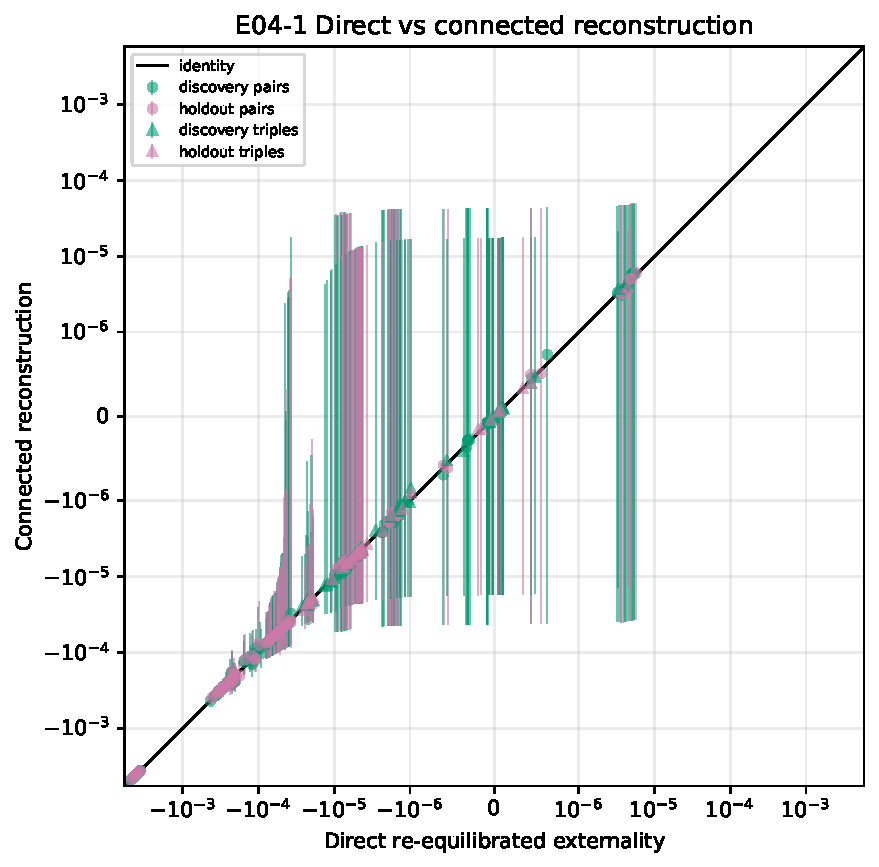
\includegraphics[width=\columnwidth]{figure_E04_1_direct_vs_reconstructed.pdf}
\caption{Direct re-equilibrated externality versus connected reconstruction
for every resolved discovery and holdout case. Error bars are conservative
combined uncertainty; the signed symlog axes retain small and negative
values. All 129 holdout cases close within five budgets.}
\label{fig:reconstruction}
\end{figure}

This agreement checks more than a final scalar. The direct route uses only
coalition vertices and M\"obius differencing. The connected route evaluates
total matrix derivatives, the complete set-partition expansion, frequency
integration, and action-hypercube quadrature. Closing the two independently
implemented paths is therefore evidence for the calculus and its numerical
implementation. It is not a causal identification theorem: both calculations
operate on the same model and action definitions.

\subsection{Why Re-Equilibration Is Material to the Calculation}

The connected anatomy distinguishes intrinsic mixed derivatives, products of
single-action feedback terms, and mixed curvature. For A7--A8 on holdout, the
median curvature contribution was $-0.00338136$ and the median feedback
contribution was $-0.000694529$, giving a median singleton-feedback adequacy
ratio of only 0.169. Thus most of this finite pair is associated with the
operating-point/network curvature that appears when dispatch and branch
reactance are changed together.

At OP00, the fully re-equilibrated A7--A8 externality is approximately
$-0.00411$, while the frozen-affine result is $-0.00065321$. The frozen
calculation therefore captures only about 15.9\% of the finite magnitude, an
underestimate of approximately $6.3\times$. Figure~\ref{fig:frozen} shows
the diagnostic for the registered exemplars. This factor belongs to A7--A8 at
the reference operating point; it is not asserted as a universal correction
factor.

\begin{figure}[t]
\centering
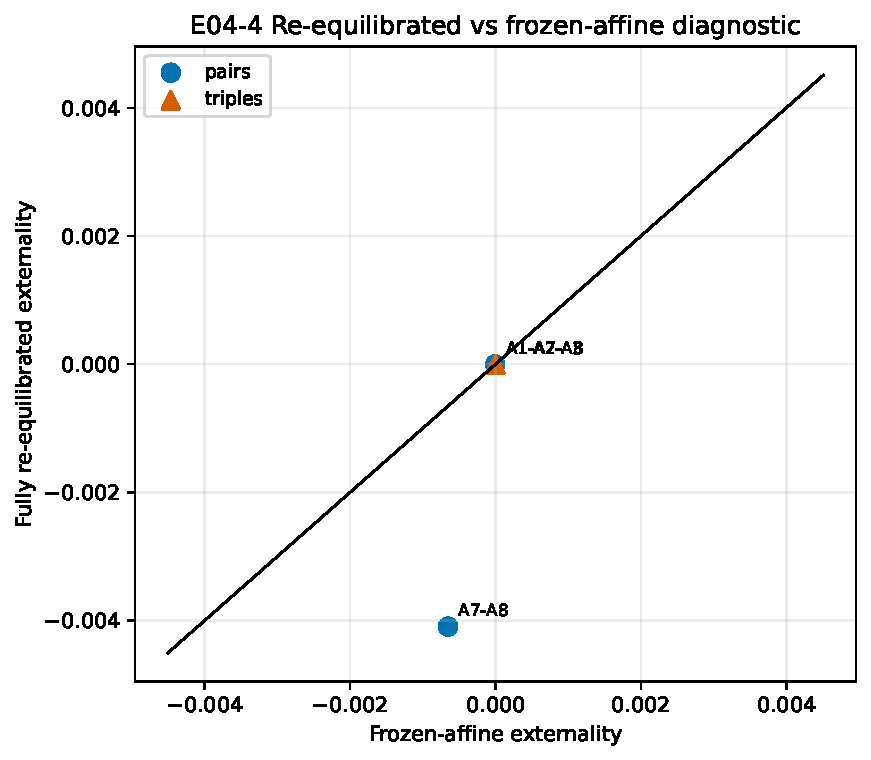
\includegraphics[width=\columnwidth]{figure_E04_4_frozen_vs_reequilibrated.pdf}
\caption{Fully re-equilibrated versus frozen-affine externality at OP00 for
registered examples. The dispatch--network pair A7--A8 lies far from the
identity line: re-equilibration increases its magnitude by about $6.3\times$.}
\label{fig:frozen}
\end{figure}

The result sharpens the comparison with local sensitivity. Higher-order
equilibrium sensitivities can be computed
\cite{nam2000eigensensitivity,zamoracardenas2013multiparameter}; the present
calculus does not claim otherwise. Its distinction is that the target object
is the exact finite coalition remainder, and that mixed curvature is retained
along the entire finite action path rather than truncated at one expansion
point.

For the resolved triples, the median adequacy of the pure-feedback
description was 0.975323, but signed terms sometimes canceled strongly.
Accordingly, component signs and magnitudes are reported directly rather than
converted into unstable percentage shares near a zero total. A large
adequacy ratio for one action family does not justify discarding curvature
for another.

\section{Exact Factor Anatomy and Pole Localization}
\subsection{Schur Closure}

The E05B holdout applied \eqref{eq:factor} to the 15 retained coalitions at 16
independent operating points. All builds were smooth-valid. The largest
pointwise log-determinant factorization residual was
$7.38964\times10^{-13}$; the largest residual after frequency integration was
$2.27374\times10^{-13}$; and the largest residual after finite M\"obius
differencing was $3.41061\times10^{-13}$. These values are consistent with
floating-point roundoff relative to the observed externalities.

The factorization answers a question that the aggregate characteristic
functional cannot: is a finite externality produced predominantly by
algebraic re-equilibration, action-dependent dynamic scaling, or pole motion?
Figure~\ref{fig:factor} reports the median holdout anatomy for four registered
examples.

\begin{figure}[t]
\centering
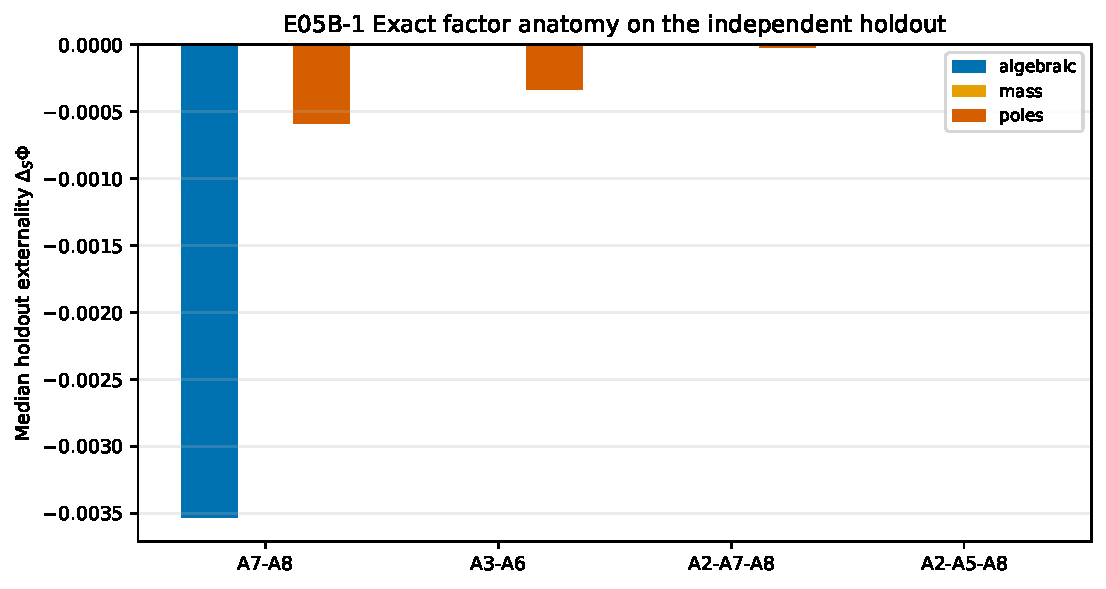
\includegraphics[width=\columnwidth]{figure_E05B_1_factor_anatomy.pdf}
\caption{Exact median holdout anatomy for registered coalitions. A7--A8 is
dominated by the algebraic factor, while A3--A6 has zero connected
algebraic/mass contribution and is pole dominated. Small triple coefficients
are retained rather than visually inflated.}
\label{fig:factor}
\end{figure}

For A7--A8, the median full externality was $-0.00411289$. Its algebraic,
mass, and pole components were $-0.00353228$, approximately zero, and
$-0.00059089$, respectively. The leading spectral interaction is therefore
largely an ac re-equilibration effect in the descriptor determinant, although
it also contains a reproducible pole component.

A3--A6 provides the complementary case. These two co-located action families
act on the bus-38 PLL and current-command bandwidths. Their connected
algebraic and mass terms are zero at the recorded precision, while the median
pole externality is $-0.00033610$. This is a direct counterexample to the idea
that every resolved log-determinant externality is merely an algebraic
power-flow artifact. Ten pairs and five triples exhibit reproducible
finite-pole externalities on the E05B holdout.

The triple results require careful language. A nonzero third-order coefficient
in $\Phi_{\mathrm{pole}}$ is a genuine third-order \emph{finite-pole
externality}: after removing all lower-order set contributions, the pole
factor remains non-additive. It does not show that three physical devices
form an isolated causal loop. Such a statement would require a frozen
localization object, a mechanism-specific intervention, and a matched negative
control, none of which is present here.

\subsection{Connected Logarithmic Derivative and Contour Moments}

Differentiating only the pole factor with respect to $s$ removes the
frequency-independent algebraic and mass factors:
\begin{equation}
\frac{\partial}{\partial s}\log\det(sI-A)
=\tr[(sI-A)^{-1}].
\label{eq:logderiv}
\end{equation}
Applying the finite connected difference to \eqref{eq:logderiv} gives a
resolvent-based description of non-additive pole displacement. Registered
closed contours then provide zeroth- and first-order moments. A certificate is
accepted only when the contour stays clear of poles at every required action
vertex, occupancy is consistent, quadrature refinement closes, and direct and
connected moments agree.

Three candidates met these conditions across all 16 holdout points: the pair
A7--A8 and triples A2--A7--A8 and A2--A5--A8. For A7--A8, the median absolute
first-moment shift was $4.74913\times10^{-3}\ \mathrm{s}^{-1}$; the median
real and imaginary components were $4.65632\times10^{-3}$ and
$-8.99434\times10^{-4}\ \mathrm{s}^{-1}$, respectively. Maximum numerical
contour error was $1.24\times10^{-15}$. Both triple candidates likewise
retained valid one-pole certificates and same-sign fraction 1.0.

The A3--A6 contour did not pass. Its maximum numerical contour error was
0.9151, leaving zero valid-resolved holdout points under the registered rule.
This negative case is retained. The factor decomposition still proves that
A3--A6 has a pole externality; it does not authorize a contour-localized pole
claim for that coalition.

\subsection{Relation to Return-Ratio, Impedance, and Spectral Methods}

Return-difference matrices and impedance Nyquist tests diagnose feedback
stability and interconnection effects
\cite{macfarlane1970return,sun2011impedance,rygg2016sequence}. They can often
be measured or assembled with fewer internal model details than
\eqref{eq:descriptor}. Proximal eigenvalue-displacement methods identify modes
whose coupling invalidates a first-order open-loop approximation
\cite{dewangan2026interaction}. That recent comparator returns converter
interaction modes from open-loop proximity and first-/second-order eigenvalue
displacement. It overlaps with the present interest in modal interaction, but
does not define a finite action-coalition M\"obius estimand, require a new AC
equilibrium at every subset vertex, separate descriptor-factor externalities,
or test the independently identified minimum-damping family. The present
method is neither its replacement nor a new stability criterion.

Its output is instead an attribution on a finite action set. The same physical
portfolio is evaluated at every subset, and inclusion--exclusion isolates what
belongs only to the joint finite action. The connected formula then states how
that set-function coefficient is assembled from total operator derivatives.
Finally, \eqref{eq:factor} asks whether the coefficient lies in algebraic
re-equilibration, mass scaling, or finite poles. These questions are
complementary to loop stability and modal proximity.

The determinant language also requires restraint. In finite non-normal
matrices, log determinants and contour moments are computational identities
under their stated regularity conditions. They do not inherit the ordering,
positivity, or causal interpretation of self-adjoint spectral-shift theory.
This study therefore uses \emph{connected pole localization}, not spectral
causality.

\section{From Dynamic Externality to Modal Materiality}
\subsection{Nominal Modal Consequence}

The E05 modal study selected three coalitions mechanically from E03/E04 before
examining any damping result: A7--A8 as the largest reproducible
curvature-dominated pair, A3--A6 as the largest reproducible
feedback-dominated pair, and A2--A7--A8 as the largest reproducible triple.
Each candidate achieved valid mode tracking at all eight holdout points, with
consistent signs.

The median finite damping externalities were
$-1.84336\times10^{-4}$ for A7--A8,
$-4.09123\times10^{-4}$ for A3--A6, and
$+1.18769\times10^{-5}$ for A2--A7--A8. A7--A8 and A3--A6 also produced
median total joint damping changes of $-0.00391371$ and $-0.00565123$,
respectively. Thus their portfolios change modal damping, but most of that
change is additive at the tracked-mode level. None of the 24 candidate/seed
points reached $|\ext{S}\zeta|\ge0.0025$. The nominal materiality claim was
therefore rejected under its preregistered rule.

This failure is not a contradiction. The characteristic functional integrates
the complete descriptor over a frequency band, while a damping gate observes
one tracked modal family. A large value of $\ext{S}\Phi$ may arise from
algebraic re-equilibration, pole motion in a well-damped family, or a
distributed collection of small shifts. Only the last stage asks whether the
non-additive effect consumes a decision-relevant margin.

\subsection{Load-Conditioned Stress}

E05C tested whether modal composition amplified as load increased toward the
first 0.85-pu voltage boundary. Eight new seeds, all 15 retained coalitions,
and nine stress levels were evaluated with 100\% valid externality and
tracking rates. The feasible endpoint multiplier ranged from 1.05225 to
1.083125 across seeds.

Define the real-part composition ratio
\begin{equation}
\rho_{\mathrm{comp}}=
\frac{\Re\{\lambda_{S}-\lambda_{S}^{(<|S|)}\}}
{\max(|\Re\{\lambda_{S}^{(<|S|)}\}|,\epsilon_\lambda)},
\label{eq:rho}
\end{equation}
where $\lambda_{S}^{(<|S|)}$ is the lower-order inclusion--exclusion
prediction and $\epsilon_\lambda$ is the registered numerical floor. The
largest observed $\rho_{\mathrm{comp}}$ was 0.00211758, and the largest
candidate median at the final stress point was 0.00197909. No point reached
the material damping threshold. There were no hard composition failures and
no 5\% screen crossings attributable to composition before the voltage
boundary. Both load-conditioned amplification and material consequence were
rejected.

Although $\rho_{\mathrm{comp}}$ was correlated with conditioning and
remaining margin, those regressions were explanatory and did not change a
candidate decision. A statistically monotone trend cannot substitute for the
frozen magnitude gate.

\subsection{Weak-Grid Attempt: Baseline Ineligibility}

Conventional short-circuit ratio (SCR) is useful context for GFL operation in
weak networks, but multi-infeed interactions can make single-POI strength
metrics incomplete \cite{xin2016gscr,nerc2017lowstrength}. Converter control
can also introduce weak-grid dynamics that require more than static strength
screening \cite{fan2019type4}. E05D therefore preregistered a grid-strength
path with an immutable eligibility rule: the empty-coalition baseline had to
retain at least 5\% damping in the true minimum-damping 0.1--30 Hz mode.

At $\kappa_{\mathrm{grid}}=1$, all eight new baselines already violated that
screen. Their minimum damping ranged from 0.0416536 to 0.0452751. The
corresponding conventional single-POI values were
SCR36=2.60275--2.64401, SCR37=2.57783--2.65366, and
SCR38=1.32141--1.40561. Because there was no eligible starting point, no safe
stress endpoint existed and no E05D coalition outcome was inspected.

The only valid status is \emph{unresolved--baseline ineligible}. It is neither
a rejection nor support of weak-grid materiality. The 5\% rule was not
changed, the stress direction was not reversed, and no replacement candidate
search was opened.

\subsection{Critical-Mode Baseline Audit}

After E05D closed, a separate descriptive audit asked why the eligibility
screen and the externality search referred to such different margins. It used
only $\kappa_{\mathrm{grid}}=1$, the eight E05D seeds, all 15 frozen E05B
coalitions, and the original A1--A8 definitions. It did not create a new gate.

For each empty baseline, the audit selected the true minimum-damping
positive-imaginary eigenvalue in 0.1--30 Hz, retained its left/right vectors,
condition number, BMAC, and state and descriptor participations, and tracked
that exact mode through every coalition subset. Global one-to-one matching
required BMAC at least 0.90, with registered 5-, 9-, and 17-point homotopies.
All 200 unique subset tracks and all 120 coalition/seed comparisons succeeded.

All eight limiting modes were synchronous-electromechanical. Their frequencies
were 1.21973--1.22906 Hz, damping ratios were 0.0416536--0.0452751, and
synchronous-machine/governor/exciter states carried
0.98619--0.98982 of normalized descriptor participation. By contrast, the 15
externality-dominant development modes were PLL/current-control families with
damping 0.49390--0.99168. Figure~\ref{fig:separation} exposes both the damping
and physical-family separation.

The limiting family is a coherent multi-machine electromechanical mode rather
than a single converter-local mode. Median descriptor endogeneity is led by
the rotor speed/angle channels of GENROU32, GENROU30, GENROU34, GENROU31, and
GENROU33; the median angle-channel shares are 0.1450, 0.0849, 0.0816, 0.0727,
and 0.0547, respectively. This state anatomy supports the family label without
promoting it to a causal intervention target.

\begin{figure*}[t]
\centering
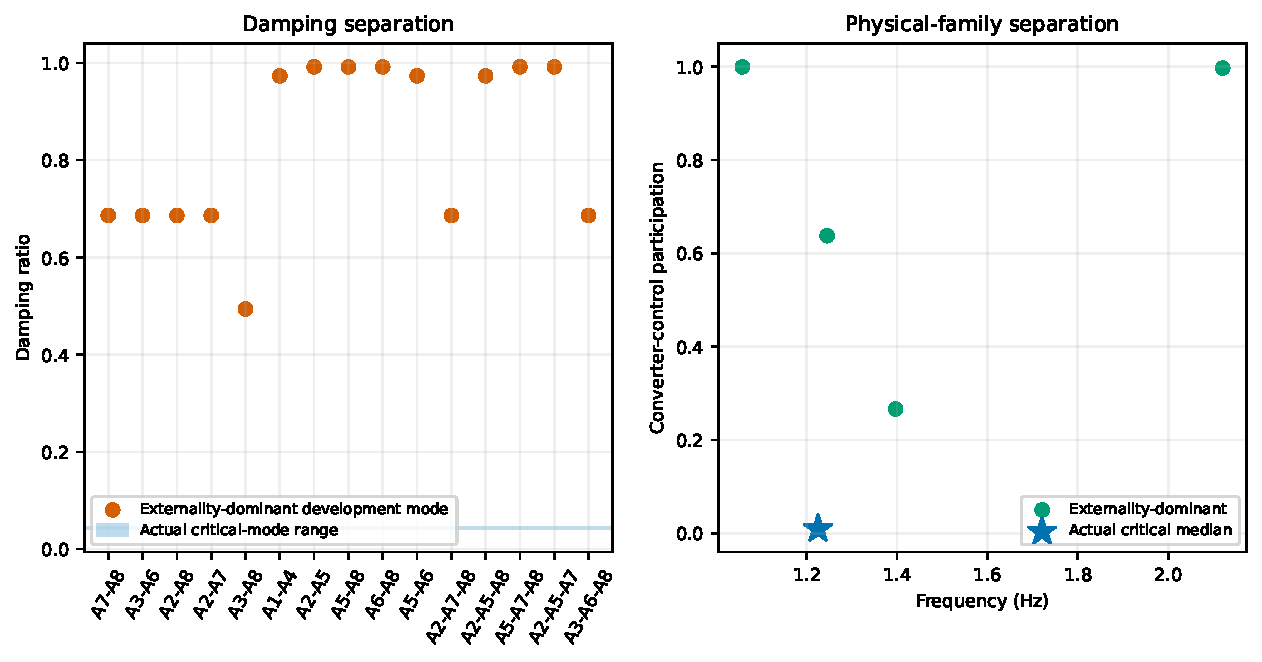
\includegraphics[width=0.94\textwidth]{figure_4_externality_vs_margin_mode.pdf}
\caption{Externality-dominant development modes versus the actual
margin-setting mode at $\kappa_{\mathrm{grid}}=1$. Left: the development
modes are much more strongly damped than the 4.17--4.53\% critical-mode band.
Right: they are converter-control/PLL dominated, whereas the critical mode is
synchronous-electromechanical near 1.22 Hz.}
\label{fig:separation}
\end{figure*}

Across all 120 coalition/seed cases, the largest critical-mode
$|\ext{S}\zeta|$ was $5.14674\times10^{-6}$. The maximum
$\rho_{\mathrm{comp}}$ was $1.39286\times10^{-4}$ for A7--A8 on seed D02,
where $\ext{\{7,8\}}\Re\lambda=4.56767\times10^{-5}\ \mathrm{s}^{-1}$.
The most stabilizing ratio was $-9.63916\times10^{-6}$ for A5--A8, and the
median absolute ratio over all cases was $6.38782\times10^{-6}$. These values
are descriptive evidence for a mode-family mismatch, not a post hoc
reinterpretation of E05D.

Table~\ref{tab:materiality} summarizes the resulting boundary. Structural
externalities survive every exactness and reproducibility check, while
operational materiality does not survive the registered consequence tests.

\begin{table}[t]
\caption{Externality Existence Versus Modal Materiality}
\label{tab:materiality}
\centering
\footnotesize
\begin{tabular}{p{0.35\columnwidth}p{0.24\columnwidth}p{0.22\columnwidth}}
\toprule
Evidence & Value & Interpretation\\
\midrule
A7--A8 spectral externality & $-0.00411$ median holdout & Exists; algebraic dominated\\
A3--A6 pole externality & $-3.36\times10^{-4}$ & Exists; pole dominated\\
Nominal $|\ext{S}\zeta|$ & $4.09\times10^{-4}$ median & Below 0.0025 gate\\
Load-stress $\rho_{\mathrm{comp}}$ & 0.00211758 maximum & No material point\\
Weak-grid campaign & 8/8 baselines below 5\% & Ineligible; unresolved\\
Critical-mode audit & $5.15\times10^{-6}$ max $|\ext{S}\zeta|$ & Below registered gate on limiting family\\
\bottomrule
\end{tabular}
\end{table}

\section{Discussion}
\subsection{What the Calculus Adds}

The central practical object is the finite coalition remainder. Suppose an
analyst plans to change a converter set point, retune a controller, and alter a
nearby network element. Standard first-order screening estimates each
increment around one baseline and then sums. The present calculation instead
asks: after every subset has moved to its own ac equilibrium and its DAE has
been rebuilt, what part of the full-portfolio characteristic change cannot be
assigned to lower-order subsets?

That question is useful even when the answer is not operationally material.
It distinguishes three failure modes of a simpler approximation:
\begin{enumerate}
    \item \emph{finite-action error}: a local Taylor model is inaccurate over
    the specified amplitude;
    \item \emph{re-equilibration error}: the operating point and algebraic
    Jacobian move jointly with the actions;
    \item \emph{interaction-order error}: pair or triple terms remain after
    all lower-order terms are removed.
\end{enumerate}
The A7--A8 result contains all three. At OP00, a frozen-affine representation
misses about 84.1\% of the finite coefficient, while exact factor anatomy
shows that its largest contribution is algebraic re-equilibration. A3--A6,
however, has a reproducible pole-only coefficient. The method thus prevents
the blanket conclusion that a characteristic externality must be merely a
power-flow artifact or a dangerous control mode.

The connected reconstruction also supplies a stringent internal check. Direct
M\"obius differencing and integrated connected traces have different numerical
error paths. Their locked-holdout agreement makes it difficult for a sign
convention, missing partition, or omitted curvature term to survive
undetected. Exact Schur closure adds a second independent identity at the
descriptor-factor level.

\subsection{Finite Portfolio Information Absent from a Baseline First-Order Screen}

A first eigenvalue sensitivity can rank actions for one mode near one
equilibrium. Higher-order and equilibrium-point sensitivities extend that
local picture \cite{nam2000eigensensitivity,zamoracardenas2013multiparameter}.
Selective modal analysis can reduce the calculation to relevant state groups
\cite{perezarriaga1982sma}. These remain the appropriate tools when the
decision question is local and the limiting modal family is known.

The finite calculus contributes when the decision variable is a named
portfolio at a non-infinitesimal amplitude. It does not approximate the
M\"obius coefficient from a derivative at zero; it evaluates the coefficient
directly and then reconstructs it by integrating the derivative over the
whole hypercube. This is why mixed re-equilibration curvature matters. The
6.3-fold A7--A8 discrepancy would not be repaired merely by better tracking of
the baseline eigenvalue.

Conversely, the critical-mode audit shows what the spectral functional can
miss if used alone: relevance to the limiting mode. The functional found
converter-control interactions reproducibly, and the pole factor verified
that some were dynamic. But these modes were strongly damped. A separate
minimum-damping search was required to show that the operative margin belonged
to a synchronous family and that the externality barely moved it. Modal
association tools---BMAC, participation, residues, condition numbers, and
homotopy---support that family identification; none is a causal proof.

\subsection{Power-System Relevance}

Three features make the experiment more than a matrix identity exercise.
First, actions are recognizable engineering changes: 20\% controller-bandwidth
adjustments, a 20-MW dispatch change, and a 10\% branch-reactance change.
Second, every coalition is required to satisfy the ac equations, dynamic
initialization, and smooth-path checks. Third, the strongest pair couples
dispatch and its incident network path, exactly the setting in which frozen
network or fixed-operating-point screening is most vulnerable.

The negative materiality result is also relevant. Interaction-detection
methods are often motivated by weak-grid risk, but interaction is not
synonymous with limiting instability. In this benchmark, conventional SCR
values provide useful context yet do not identify which modal family sets the
5\% screen. The critical mode is synchronous-electromechanical despite the
presence of three GFL plants and conspicuous converter-mode externalities.
Planning studies should therefore distinguish at least three questions:
\begin{enumerate}
    \item Is a portfolio non-additive in a chosen dynamic functional?
    \item Does the non-additivity arise in algebraic coordinates or finite
    poles?
    \item Does it materially change the mode or constraint that limits the
    operating decision?
\end{enumerate}
The first two can be positive while the third is negative.

\subsection{Limitations}

The action space contains eight coordinates and only one matched IEEE 39-bus
GFL testbed. The results establish reproducible existence, not prevalence
across converter vendors, control architectures, larger networks, or action
amplitudes. The three converter models share a common class. Grid-forming
controls, hybrid populations, protection and saturation events, unbalanced
dynamics, and topology-discontinuous actions remain outside scope.

The spectral functional is dimensionless and band dependent. Its sign and
magnitude are not direct measures of damping, instability probability,
energy, or economic cost. The normalized logarithmic frequency weight and
0.1--30 Hz band were frozen before the campaign, but another defensible
functional may rank coalitions differently.

The finite-to-connected identity requires smooth re-equilibrated interpolation
throughout the hypercube. It does not cover a path that crosses a power-flow
bifurcation, limiter discontinuity, state-dimension change, or singular
algebraic Jacobian. The exact Schur anatomy further assumes index-one behavior,
nonsingular $g_y$, and a nonsingular registered dynamic mass block. Contour
localization is conditional on pole-free boundaries and numerical occupancy
certificates; A3--A6 demonstrates that a pole externality may exist even when
a selected contour cannot certify its localized moment.

The materiality ladder is deliberately narrow. The 0.0025 damping-externality
threshold and 5\% screen are preregistered study rules, not universal
standards. E05C ended at a voltage boundary before finding material
composition. E05D could not start because all empty baselines were already
below the screen; it therefore leaves weak-grid materiality unresolved. No
coalition result from E05D was viewed.

Finally, no cycle or SCC localization, mechanism-targeted correction,
matched-cost negative control, nonlinear time-domain consequence, or blind EMT
transfer was performed. E02C validates the benchmark infrastructure only.
Consequently, this paper does not offer an industrial mitigation or claim that
a particular interaction graph is causal.

\subsection{Implications for Future Use}

The terminal findings suggest a disciplined workflow for other systems when
finite portfolio composition is the decision question.
First, define finite actions in physical units and solve every coalition
vertex. Second, resolve direct externalities against numerical uncertainty.
Third, use connected reconstruction as an implementation and anatomy check.
Fourth, split algebraic and pole factors exactly. Fifth, identify the actual
constraint-setting modal family independently of the externality search.
Only if the same family carries a material, reproducible finite effect should
an intervention experiment be designed.

This ordering limits unnecessary controller surgery. In the present testbed,
the descriptive audit explains why further tuning of the externality-dominant
converter modes would not answer the registered stability-margin question.
The correct terminal outcome is a boundary statement, not a new stress search.

\section{Conclusion}

This paper introduced a finite connected intervention calculus for
converter-rich power-system DAEs. The defining choice is physical
re-equilibration: each subset of a finite action portfolio receives its own ac
solution, dynamic initialization, and descriptor operator. Direct M\"obius
differences isolate pair and triple externalities, and connected total
derivatives reconstruct them over the full action hypercube.

The registered IEEE 39-bus campaign supports five bounded conclusions.
Finite pair and genuine third-order externalities exist reproducibly. The
connected reconstruction closes all locked-holdout cases within five
conservative uncertainty budgets. Exact Schur anatomy separates algebraic,
mass-scaling, and finite-pole contributions to roundoff. Reproducible
finite-pole externalities exist, and certified contours localize pole motion
for three retained coalitions. Re-equilibration can be quantitatively
decisive: the frozen-affine approximation underestimates A7--A8 by about
$6.3\times$ at the OP00 reference point.

The experiment also establishes a firm limit. None of the selected
externalities met the preregistered nominal or load-conditioned damping
materiality criteria. The weak-grid test was baseline-ineligible and remains
unresolved. A separate audit showed why: the externality-dominant modes are
well-damped converter-control families, whereas the actual limiting mode is a
roughly 1.22-Hz synchronous-electromechanical family with only microunit-scale
finite damping composition.

The resulting conclusion is deliberately narrower than an interaction-based
stability claim: finite dynamic externalities can be real, higher order, and
reproducible without materially consuming the system's registered modal
margin. Detecting interaction structure is therefore a useful diagnostic step
when finite portfolio composition is the decision question, but it is not a
substitute for identifying
the constraint-setting mode or for demonstrating a mechanism-specific
intervention.


\section*{Data and Code Availability}
The frozen protocols, manifests, source code, machine-readable tables,
failure ledgers, and figure-generating inputs used in this paper are included
with the review package. Each terminal experiment records source and input
hashes. The E05D weak-grid package is retained unchanged, and the descriptive
critical-mode audit is stored separately so that it cannot alter a registered
gate.

\section*{Ethics, Contributions, Funding, and Competing Interests}
No human participants, animals, or personal data were involved. Author names
and CRediT roles are withheld for double-blind review and must be completed at
submission. Funding and competing-interest declarations are likewise withheld
during review and must be supplied by the authors before publication.

\section*{Generative-AI Disclosure}
A generative-AI coding assistant was used to help organize evidence, draft
prose, and check software artifacts. All numerical claims were taken from
frozen, executable experiment outputs; the authors are responsible for the
analysis, verification, citations, and final text.

\balance
\bibliographystyle{IEEEtran}
\bibliography{references}

\end{document}
